\section{Aufbau und Vorbereitung}

Im letzten Versuch wird das Verhalten gekoppelter Pendel untersucht. Der Aufbau besteht aus zwei mit einer Feder gekoppelten Stabpendeln, an denen jeweils eine Massescheibe angebracht ist.
Bevor man die Pendel koppelt, muss jedoch gesichert sein, dass die Pendel sich auch identisch verhalten.
Dazu werden zunächst der Dreh- und Massenpunkt festgelegt und dann die Periodendauern je Pendel gemessen und nach linearer Regression verglichen.

\begin{align}
    l &= \SI{80}{cm} \\
    L &= \SI{111}{cm} \\
    a &= \SI{31}{cm} \\
    m_{\text{Massescheibe}} &= \SI{1221}{g}
\end{align}

\begin{table}[h!]
    \begin{center}
        \caption{Zeiten für unterschiedliche Periodendauern beider Pendel}
        \begin{tabular}{ccc}
            \hline
            Anzahl Perioden & Zeit linkes Pendel in $\SI{}{s}$ & Zeit rechtes Pendel in $\SI{}{s}$ \\
            \hline
            3  & $\SI{5,51}{}$ & $\SI{5,36}{}$ \\
            5  & $\SI{9,09}{}$ & $\SI{8,84}{}$  \\
            7  & $\SI{12,53}{}$ & $\SI{12,51}{}$  \\
            9  & $\SI{15,98}{}$ & $\SI{16,08}{}$ \\
            \hline
            \label{tab:Schwingungen-Pendel-einzeln}
        \end{tabular}
    \end{center}
\end{table}

\begin{figure}[h!]
    \centering
    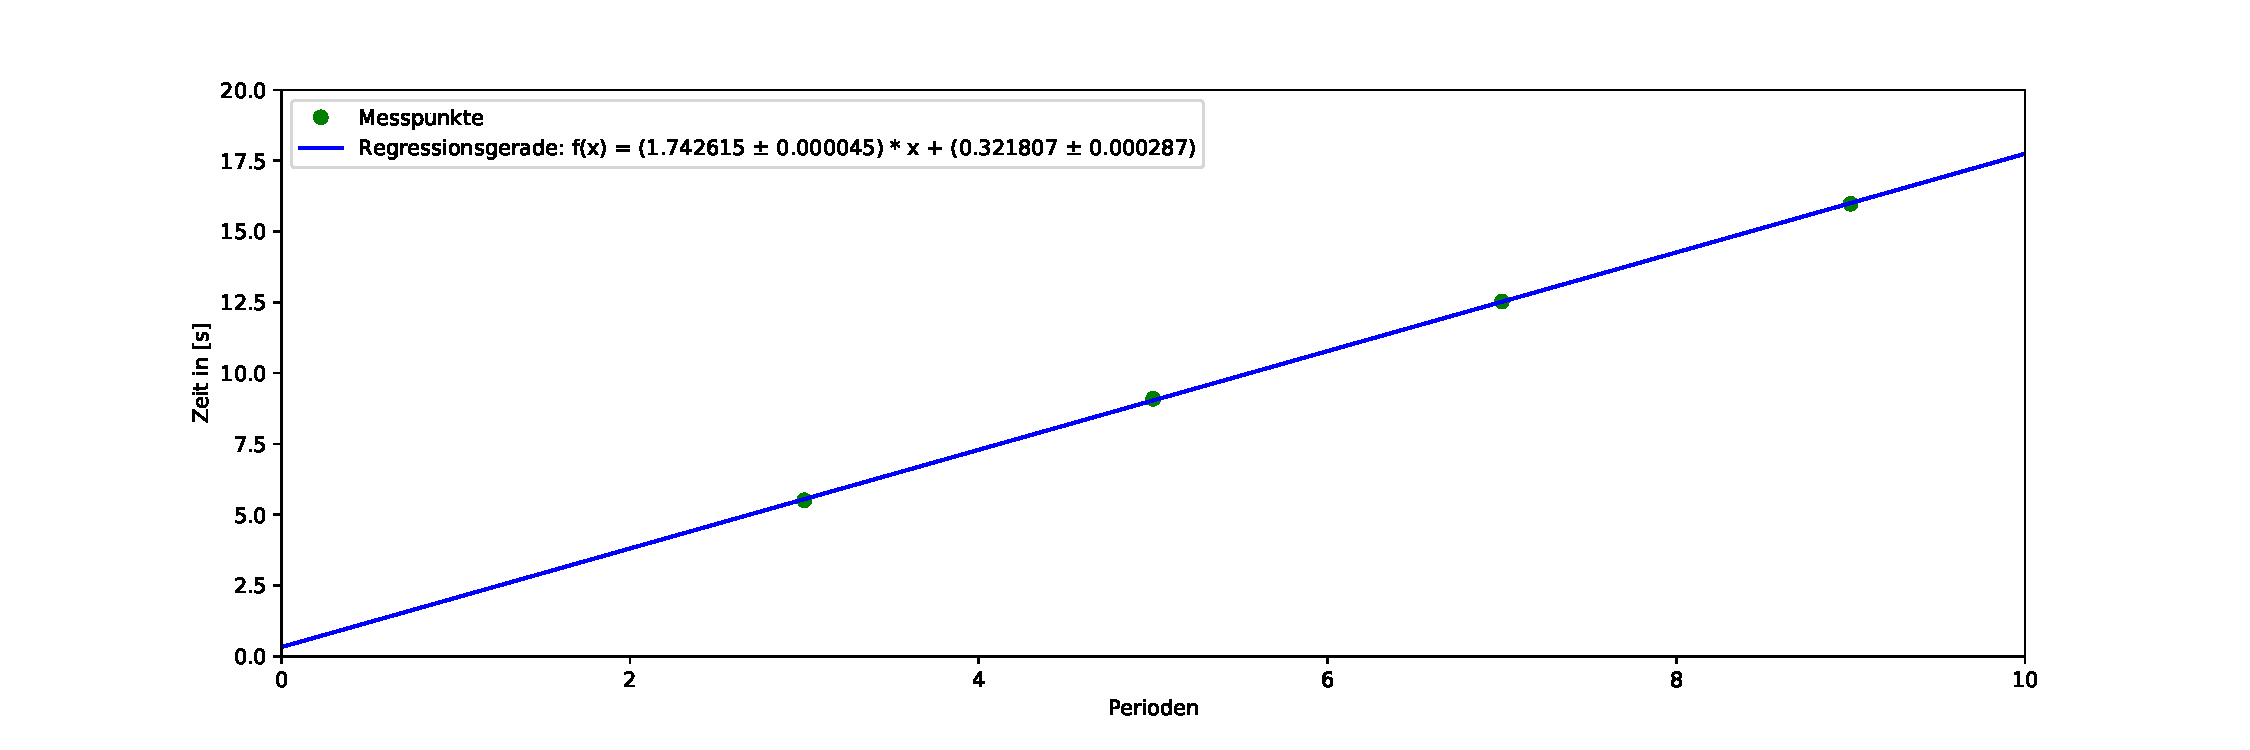
\includegraphics[scale=0.4]{./Pendel/Protokoll/fig/Koppelpendel_Regression_1.pdf}
    \caption{Plot der Messpunkte und der Regression für das linke Pendel}
    \label{fig:Reg_links}
\end{figure}

\begin{figure}[h!]
    \centering
    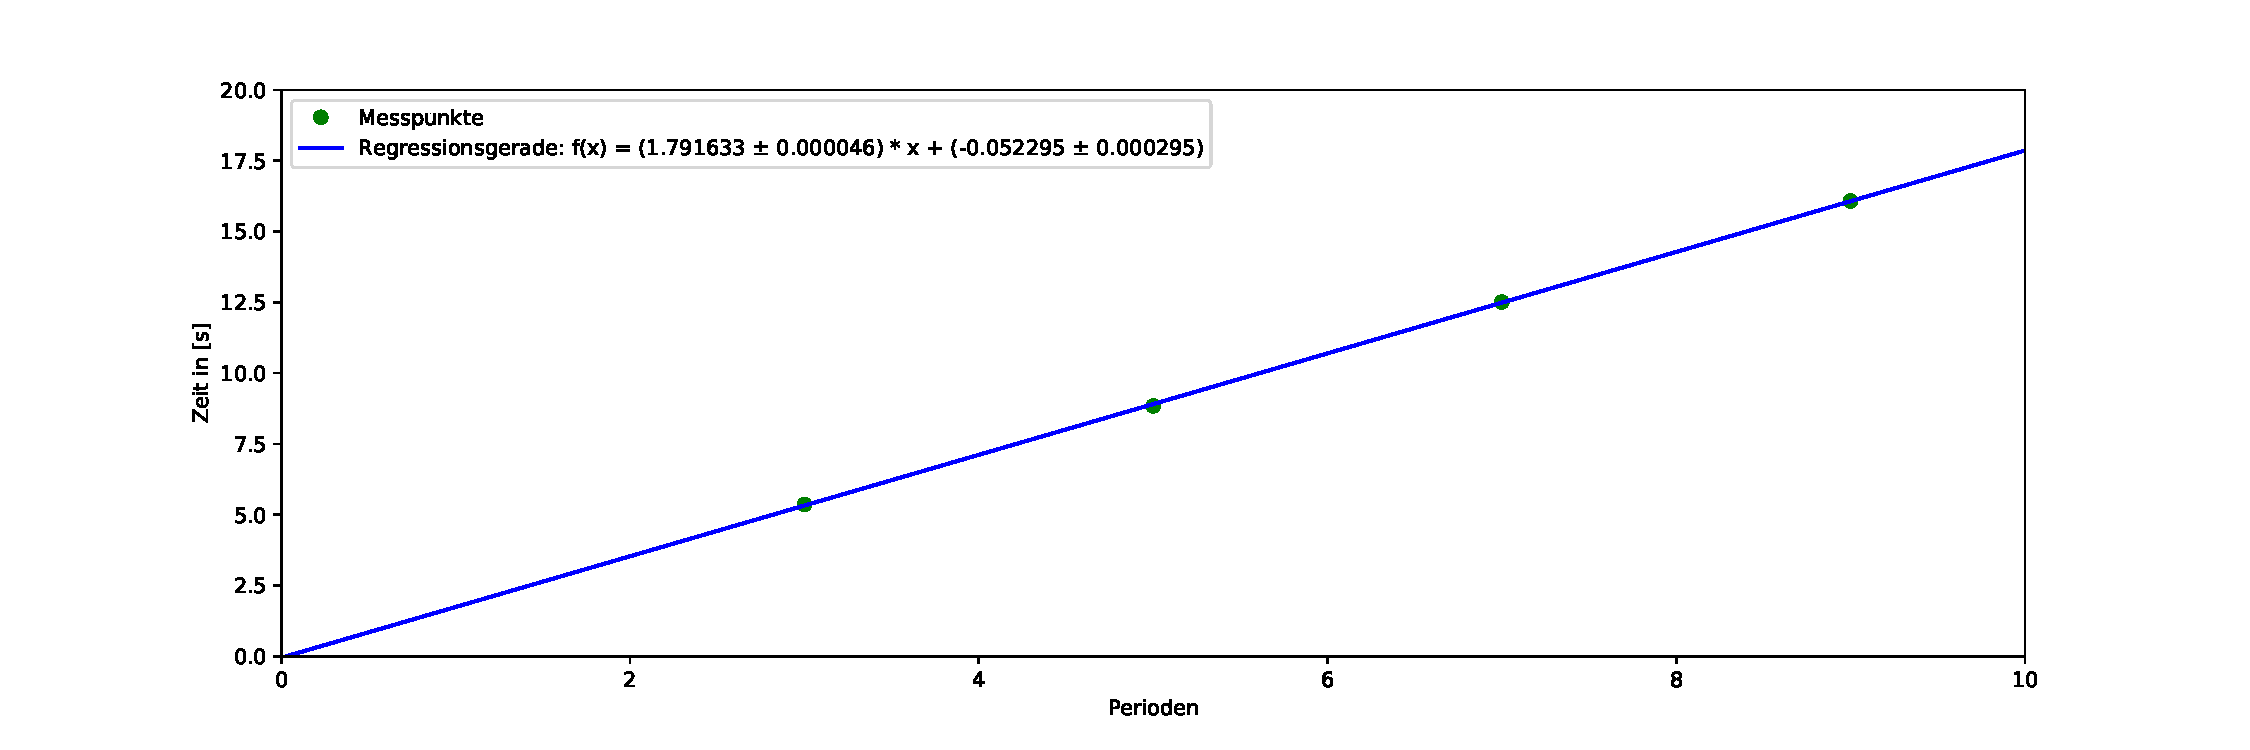
\includegraphics[scale=0.4]{./Pendel/Protokoll/fig/Koppelpendel_Regression_2.pdf}
    \caption{Plot der Messpunkte und der Regression für das rechte Pendel}
    \label{fig:Reg_rechts}
\end{figure}

\begin{table}[h!]
    \begin{center}
        \caption{Parameter lineare Regression}
        \begin{tabular}{ccc}
            \hline
            Pendel             & $m$ in $\SI{}{s}$ & $c$ in $\SI{}{s}$ \\
            \hline
            links              & $\SI{1,66(2)}{}$ & $\SI{0,8(130)}{}$ \\
            rechts             & $\SI{1,71(21)}{}$ & $\SI{0,45(135)}{}$  \\
            \hline
            Mittelwert         & $\SI{1.69(21)}{}$ & $\SI{0,063(132)}{}$ \\
            \hline
            \label{tab:Schwingungen-einzeln-Regression}
        \end{tabular}
    \end{center}
\end{table}


Da die Parameter des linken und des rechten Pendels nur gering von einander abweichen, kann man die beiden Pendel als identisch ansehen.


\clearpage

\section{Fundamentalschwingung}

Zur Analyse der Fundamentalschwingung werden die Pendel nun mit einer geeigneten Feder verbunden und die Periodendauer von Hand per Stoppuhr gemessen.
Geeignet bedeutet hier, dass die Federkonstante nicht zu groß sein sollte, da die Pendel sonst so schnell schwingen, dass die Zeit nicht mehr akkurat gestoppt werden kann.
Es wurde für zwei Koppellängen gemessen, wobei "Koppellänge" den Abstand ziwschen Drehpunkt und Federbefestigung bezeichnet.

\section{Auswertung}

\begin{table}[h!]
    \begin{center}
        \caption{Schwingungsdauern in $\SI{}{s}$}
        \begin{tabular}{cccc}
            \hline
            Koppellänge in $\SI{}{cm}$ & Periodenanzahl & gleichphasig   & gegenphasig    \\
            \hline
            \multirow{4}{*}{31}        & 3              & $\SI{5,37}{}$  & $\SI{4,70}{}$  \\
                                       & 5              & $\SI{8,79}{}$  & $\SI{7,90}{}$  \\
                                       & 7              & $\SI{12,29}{}$ & $\SI{10,83}{}$ \\
                                       & 9              & $\SI{15,9}{}$ & $\SI{14,03}{}$ \\
            \hline
            \multirow{4}{*}{28}        & 3              & $\SI{5,40}{}$  & $\SI{4,82}{}$  \\
                                       & 5              & $\SI{8,85}{}$  & $\SI{8,00}{}$  \\
                                       & 7              & $\SI{12,27}{}$ & $\SI{11,02}{}$ \\
                                       & 9              & $\SI{15,96}{}$ & $\SI{14,11}{}$ \\
            \hline
            \label{tab:Koppellaenge-Messwerte}
        \end{tabular}
    \end{center}
\end{table}

Die Auswertung geschieht erneut über Regression.

\begin{figure}[h!]{}
    \begin{center}
        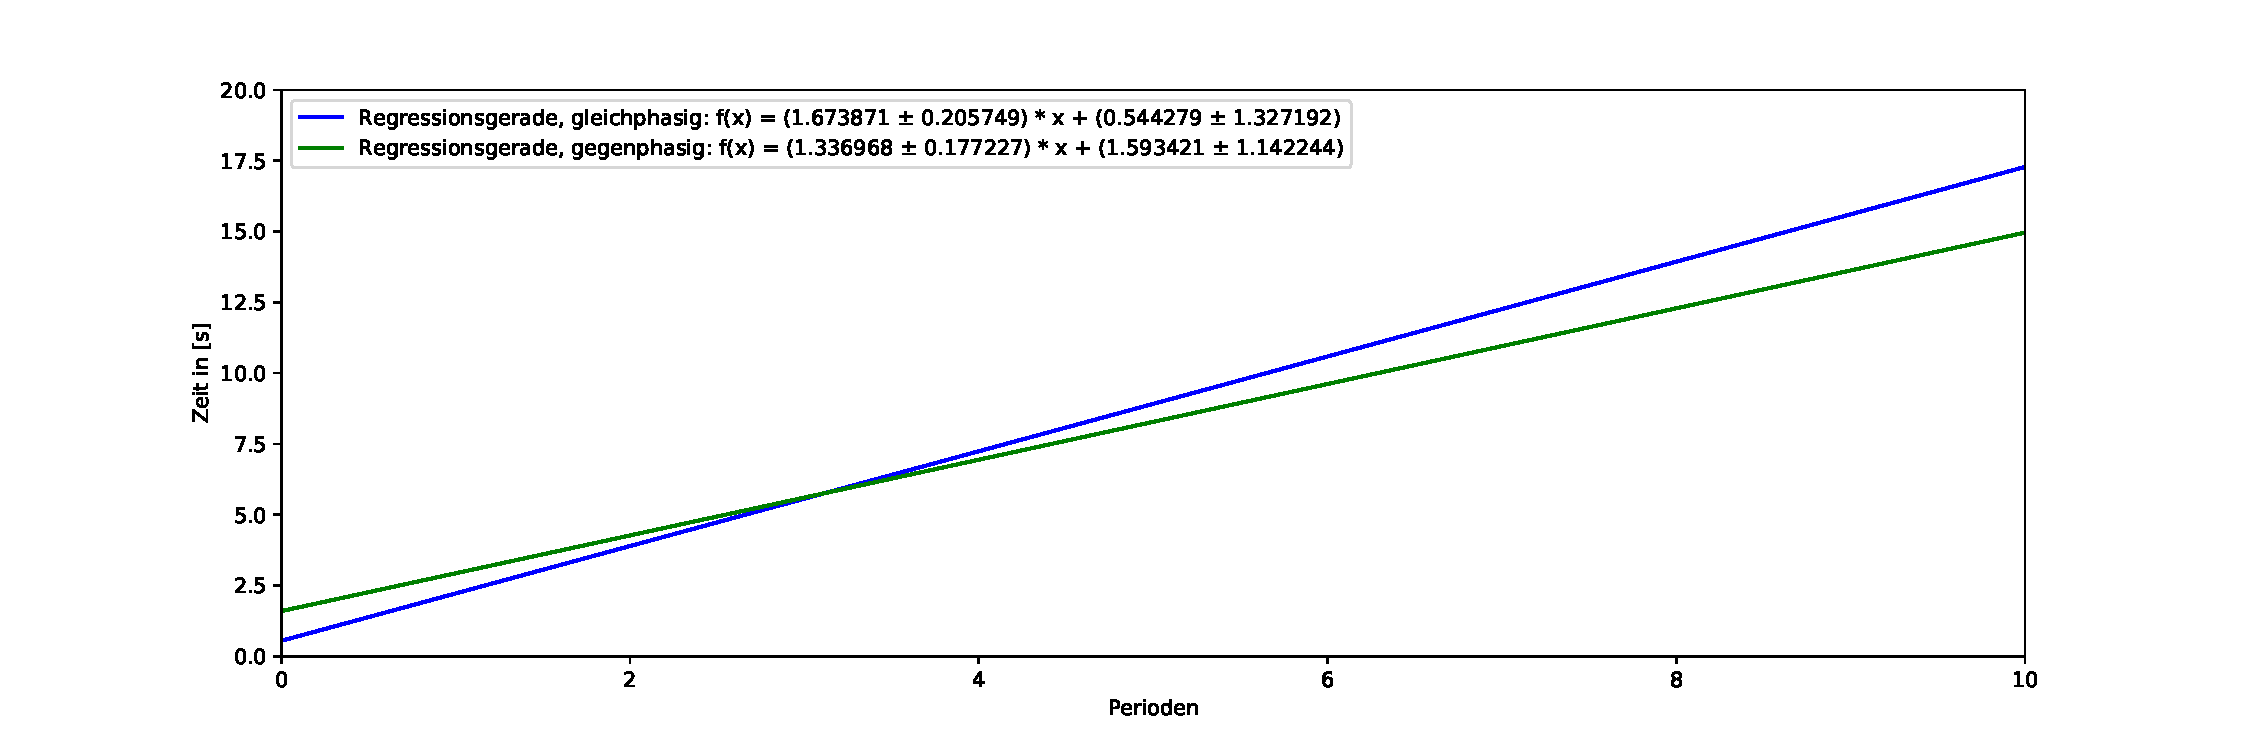
\includegraphics[scale = 0.4]{./Pendel/Protokoll/fig/Koppelpendel_Regression_3.pdf}
        \caption{Regression der Schwingungsdauern der gekoppelten Oszillatoren,  Kopplungslänge 31cm}
        \label{fig:Schwingungsdauern-gekoppelte-Oszillatoren1}
    \end{center}
\end{figure}

\begin{figure}[h!]{}
    \begin{center}
        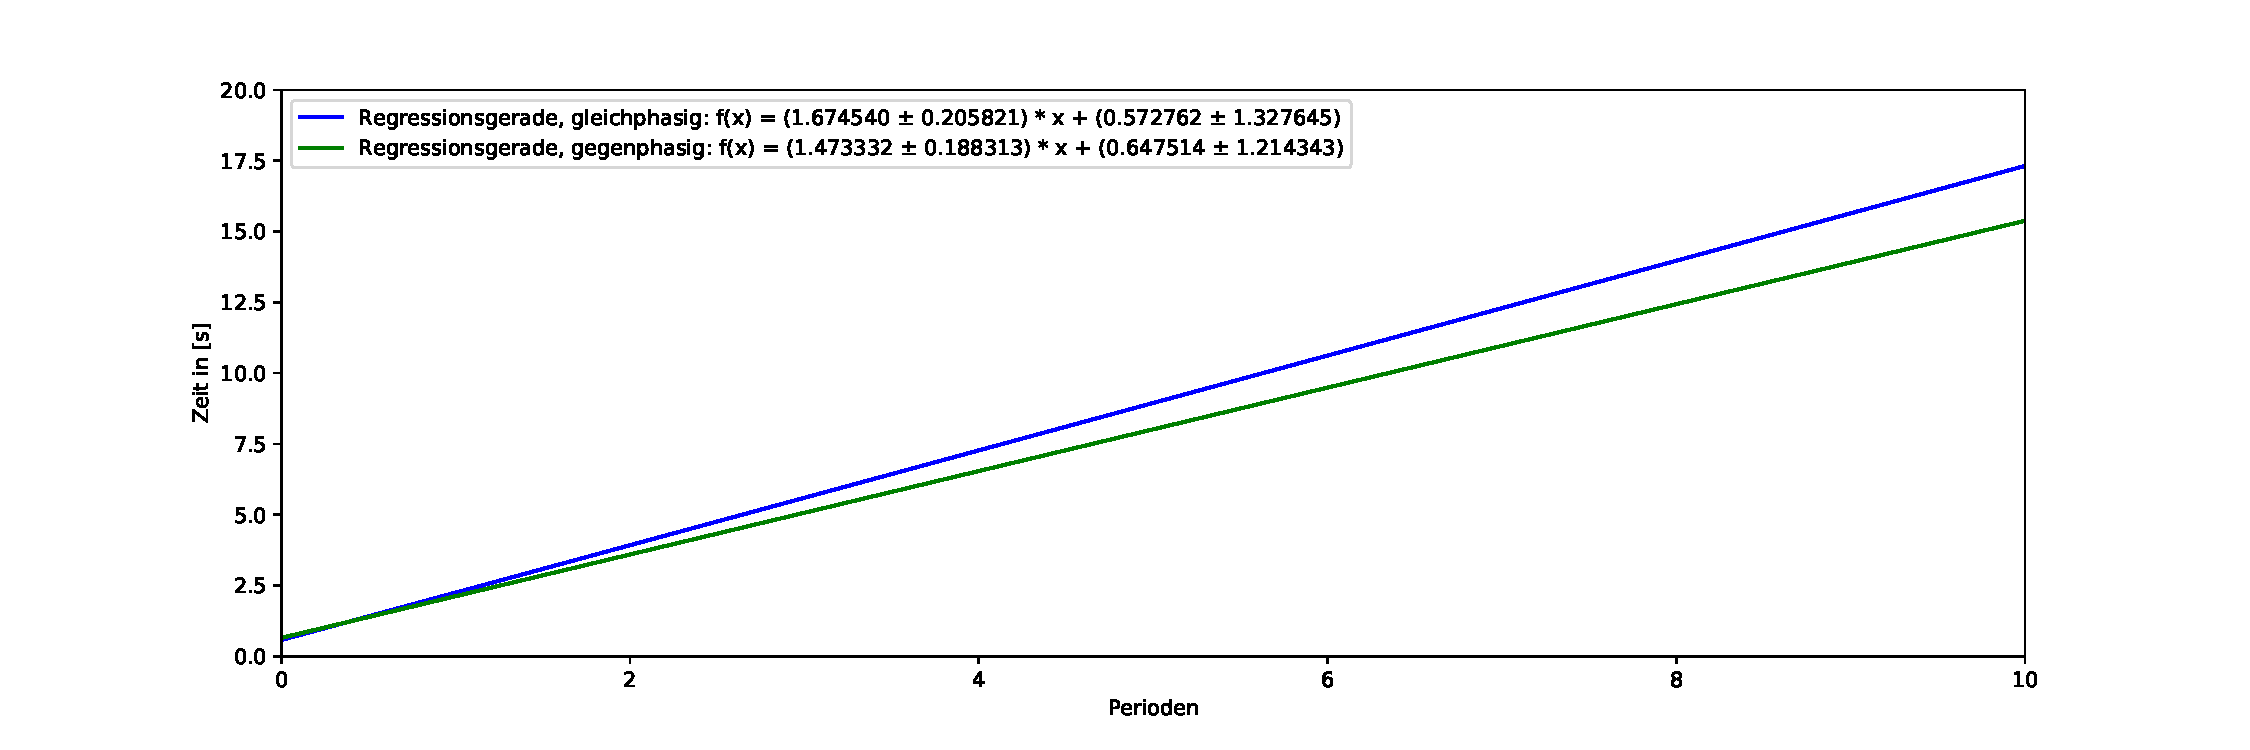
\includegraphics[scale=0.4]{./Pendel/Protokoll/fig/Koppelpendel_Regression_4.pdf}
        \caption{Regression der Schwingungsdauern der gekoppelten Oszillatoren, Kopplungslänge 28cm}
        \label{fig:Schwingungsdauern-gekoppelte-Oszillatoren2}
    \end{center}
\end{figure}


\begin{table}[h!]
    \begin{center}
        \caption{Schwingungsdauern in $\SI{}{s}$}
        \begin{tabular}{cccc}
            \hline
            Koppellänge in $\SI{}{cm}$ & Schwingungsform & m in $\SI{}{s}$   & c in $\SI{}{s}$ \\
            \hline
            \multirow{4}{*}{31}        & gleichphasig    & $\SI{1,67(21)}{}$ & $\SI{0,54(133)}{}$  \\
                                       & gegenphasig     & $\SI{1,34(18)}{}$ & $\SI{1,59(114)}{}$  \\
            \hline
            \multirow{4}{*}{28}        & gleichphasig    & $\SI{1,68(21)}{}$ & $\SI{0,57(133)}{}$  \\
                                       & gegenphasig     & $\SI{1,47(19)}{}$ & $\SI{0,65(121)}{}$  \\
            \hline
            \label{tab:Koppellaenge-Regressionswerte}
        \end{tabular}
    \end{center}
\end{table}

Vergleicht man die Messwerte für die gekoppelten Pendel mit denen der einzelnen Pendel, zeigt sich, dass bei gleichphasiger Schwingung kaum ein Unterschied vorhanden ist, während sich die Werte für die gegenphasige Schwingung deutlich von denen der einzelnen Pendel unterscheiden.
Dies ist dadurch zu erklären, dass die Feder bei gleichphasiger Schwingung nicht gedehnt wird und daher keinen signifikanten Einfluss auf das Verhalten der Pendel nimmt. Bei der gegenphasigen Schwingung wird die Feder jedoch immer wieder gestreckt und gestaucht, was das Schwingungsverhalten signifikant beeinflusst.

\section{Andersweitige Bestimmung der Federkonstante}

Im diesem Versuchteil soll die Federkonstante der vorher verwendeten Feder jeweils einmal statisch und dynamisch bestimmt werden.
Für die statische Methode wird die Feder durch das Anhängen unterschiedlich schwerer Gewichte unterschiedlich stark aus ihrer Ruheposition ausgelenkt.

\begin{table}[h!]
    \begin{center}
        \caption{statische Bestimmung der Feederkonstante}
        \begin{tabular}{cccc}
            \hline
            Gewicht in $\SI{}{g}$ & Länge der Feder in $\SI{}{cm}$ \\
            \hline
            $\SI{0}{}$ & $\SI{53,3}{}$  \\
            $\SI{100}{}$ & $\SI{57}{}$ \\
            $\SI{200}{}$ & $\SI{61,1}{}$ \\
            $\SI{500}{}$ & $\SI{72,7}{}$ \\
            \hline
            \label{tab:Feder-statisch-Messwerte}
        \end{tabular}
    \end{center}
\end{table}

Für die dynamische Methode wird ein Gewicht von blubba an die Feder gehängt und dann in Schwinung versetzt. Wie in blubba wurde die Schwingungsdauer per Stoppuhr erfasst.

\begin{table}[h!]
    \begin{center}
        \caption{dynamische Bestimmung der Federkonstante}
        \begin{tabular}{cccc}
            \hline
            Periodenanzahl & Schwingungsdauer in $\SI{}{s}$ \\
            \hline
            $\SI{10}{}$ & $\SI{6.19}{}$  \\
            $\SI{20}{}$ & $\SI{11.99}{}$  \\
            $\SI{30}{}$ & $\SI{17.65}{}$  \\
            
            \hline
            \label{tab:Feder-dynamisch-Messwerte}
        \end{tabular}
    \end{center}
\end{table}


Auswertung

Die Auswertung passiert erneut über Regression.


\begin{figure}[h!]{}
    \begin{center}
        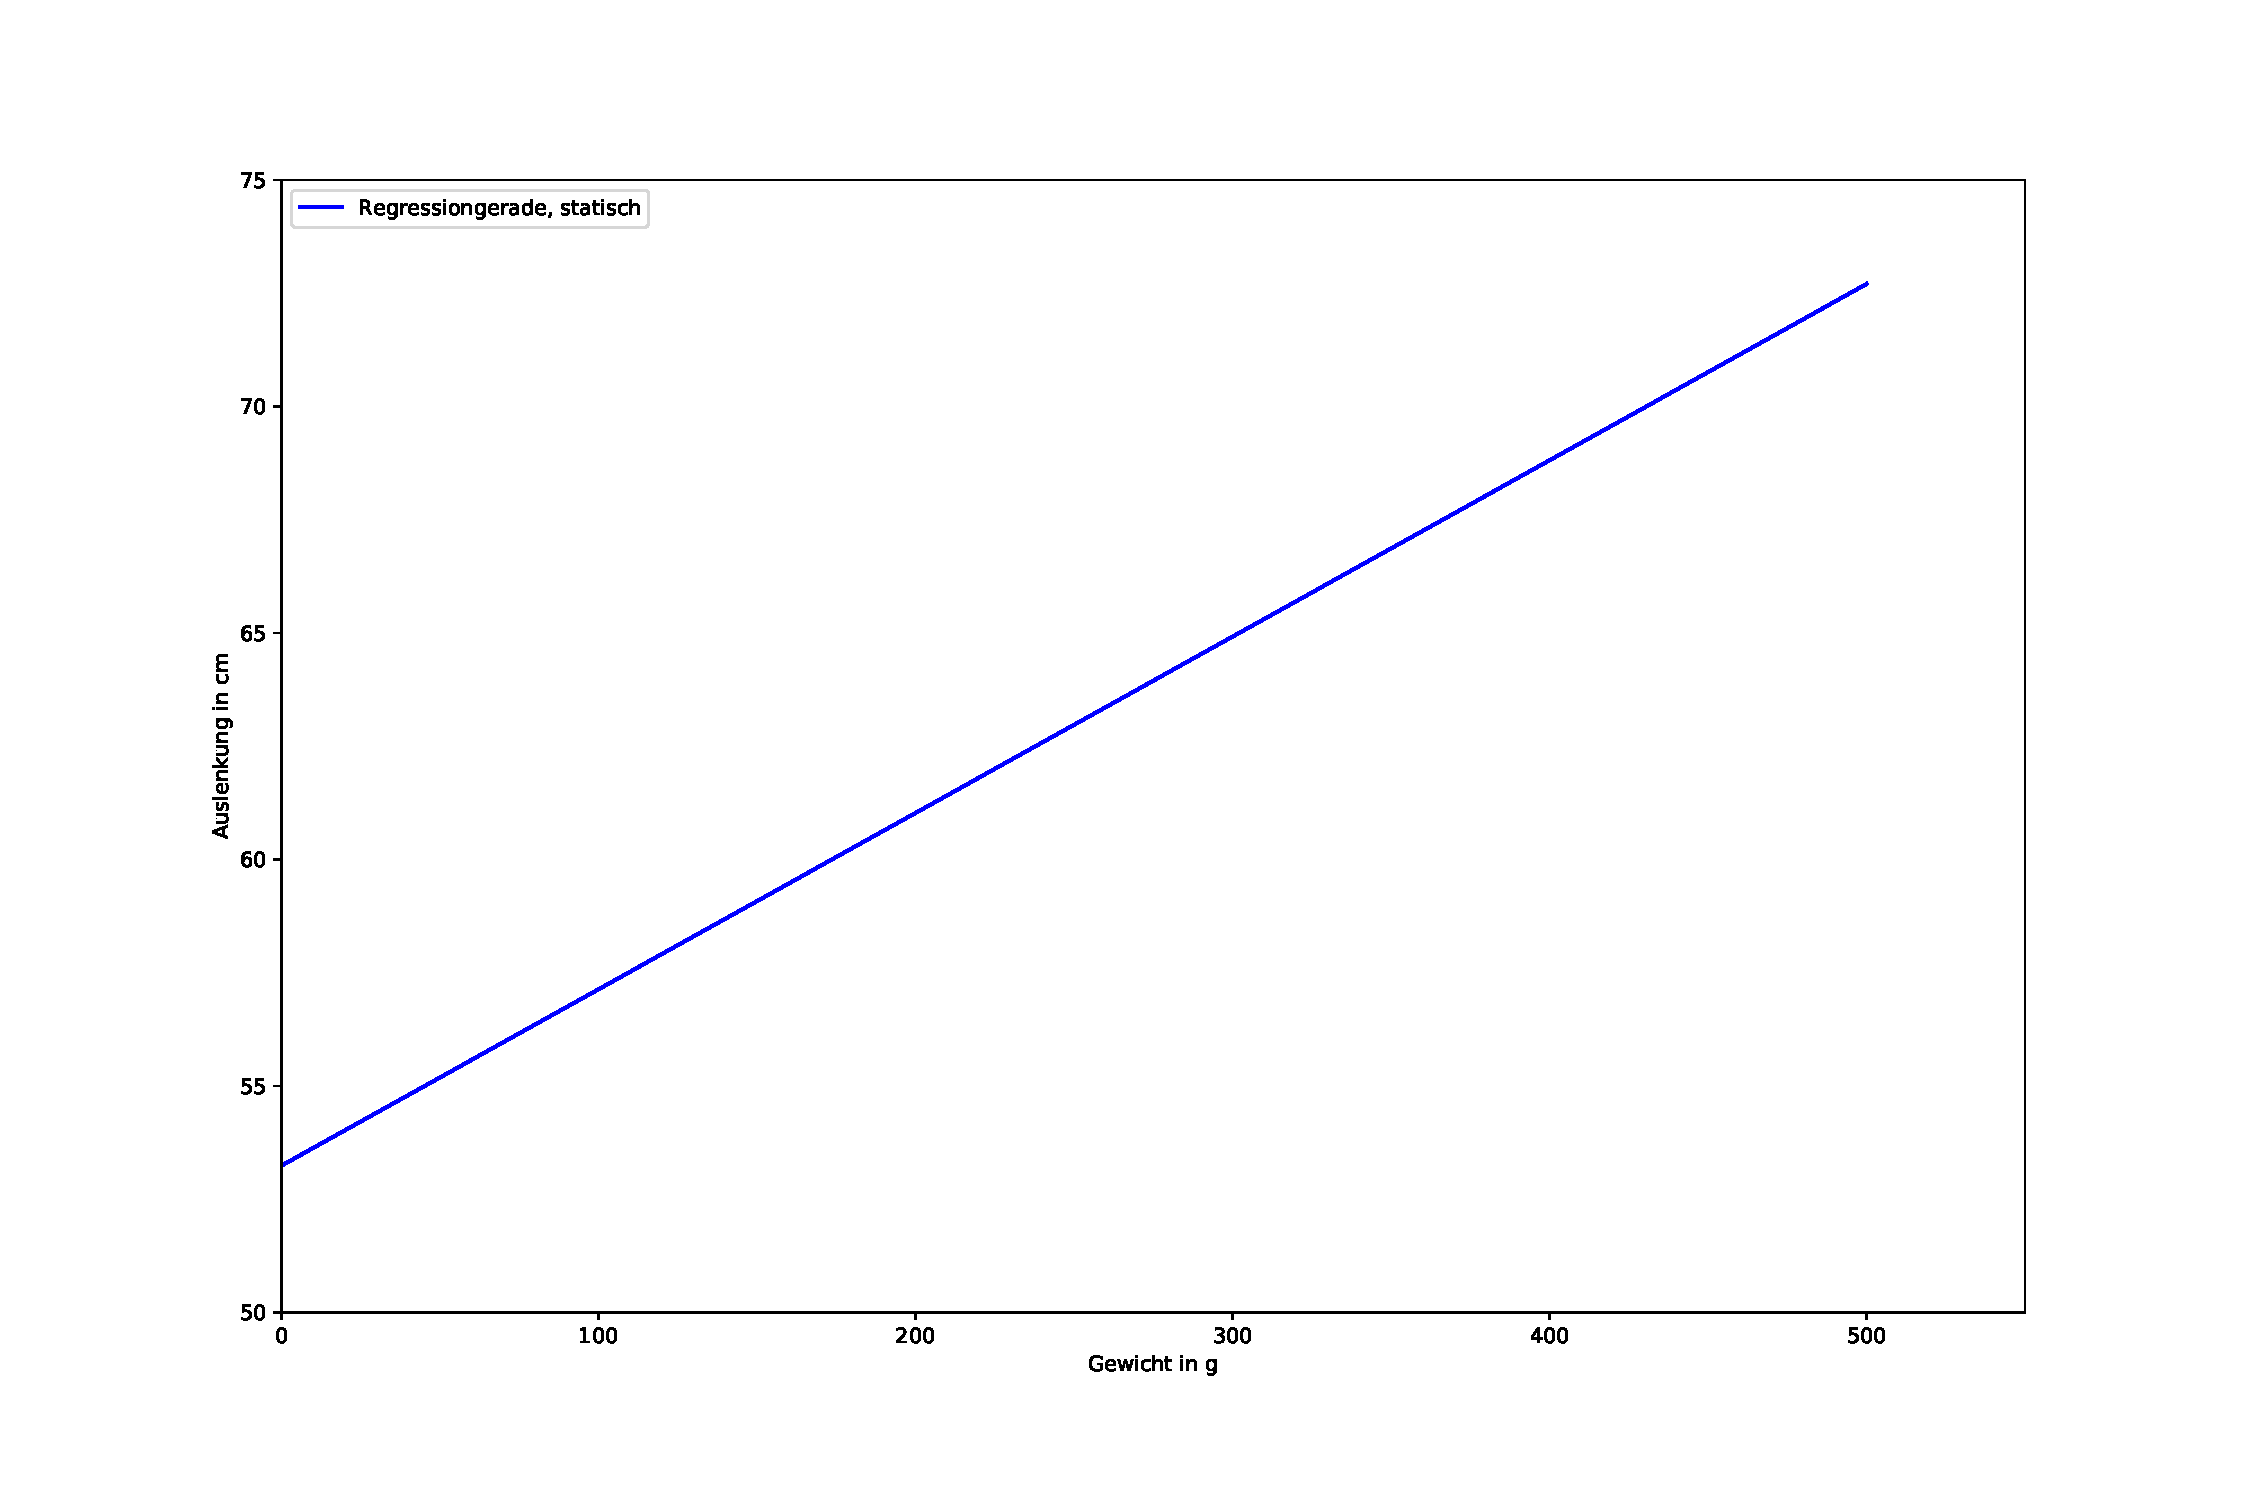
\includegraphics[scale = 0.4]{./Pendel/Protokoll/fig/Federkonstante_1.pdf}
        \caption{Regression der Schwingungsdauern der gekoppelten Oszillatoren,  Kopplungslänge 31cm}
        \label{fig:Schwingungsdauern-gekoppelte-Oszillatoren1}
    \end{center}
\end{figure}

\begin{figure}[h!]{}
    \begin{center}
        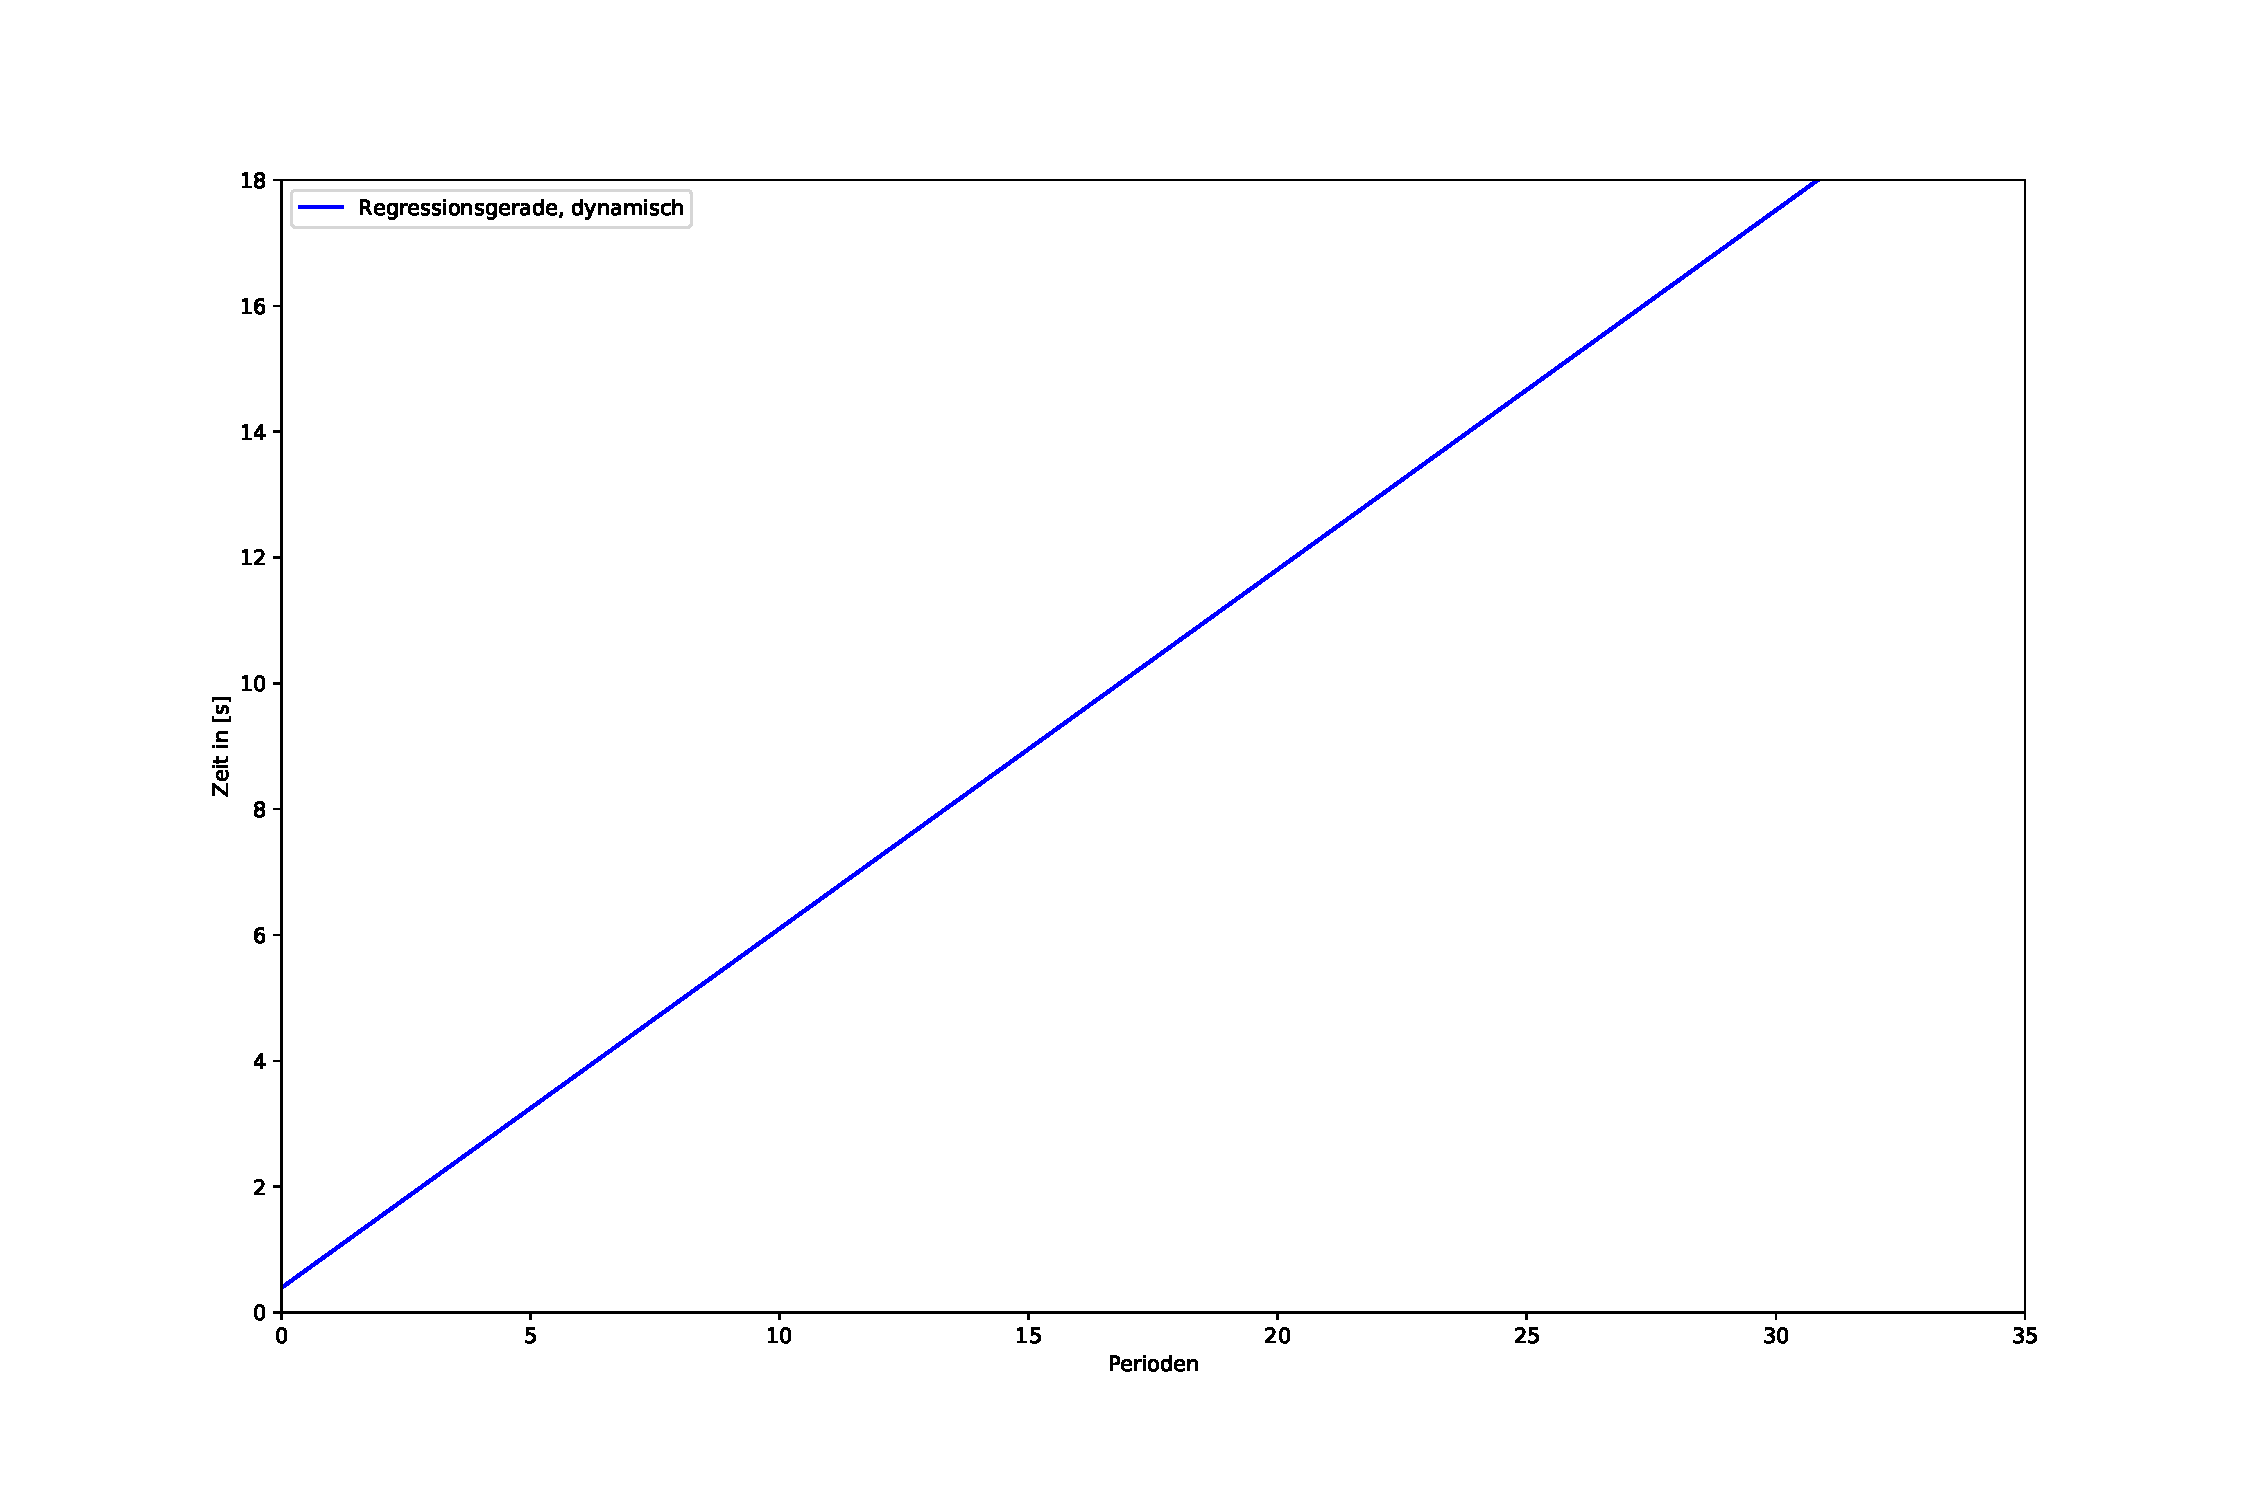
\includegraphics[scale=0.4]{./Pendel/Protokoll/fig/Federkonstante_2.pdf}
        \caption{Regression der Schwingungsdauern der gekoppelten Oszillatoren, Kopplungslänge 28cm}
        \label{fig:Schwingungsdauern-gekoppelte-Oszillatoren2}
    \end{center}
\end{figure}

Statisch ergibt sich mit eine Federkonstante von

\begin{equation}
    D = \frac{m \cdot g}{x} =\SI{17,21}{\frac{N}{m}} = 
\end{equation}

Dynamisch ergibt sich eine Federkonstante von

\begin{equation}
    D = 4 \cdot \pi^2 \frac{m}{T^2} = \SI{60,75}{\frac{N}{m}}.
\end{equation}

Schwingungs- und Schwebungsdauer gekoppelter Oszillatoren

Nun werden noch die Schwingungs- und die Schwebungsdauer des gekoppelten Pendels aus blubba gemessen.
Dazu wird ein Pendel ausgelenkt, während das andere in Ruhe verbleibt.

\begin{table}[h!]
    \begin{center}
        \caption{Schwingungs- und Schwebungsdauer}
        \begin{tabular}{cccc}
            \hline
            Periodenanzahl & Schwingungsdauer in $\SI{}{s}$ & Schwebungsdauer in $\SI{}{s}$ \\
            \hline
            $\SI{}{}$ & $\SI{}{}$ & $\SI{}{}$ \\
            $\SI{3}{}$ & $\SI{5,08 }{}$ & $\SI{44,19 }{}$ \\
            $\SI{5}{}$ & $\SI{8,59 }{}$ & $\SI{115,41}{}$ \\
            $\SI{7}{}$ & $\SI{11,70}{}$ & $\SI{144,49}{}$ \\
            $\SI{9}{}$ & $\SI{15,74}{}$ &  \\
            \hline
            \label{tab:Feder-dynamisch-Messwerte}
        \end{tabular}
    \end{center}
\end{table}

Zur Auswertung wurde erneut Regression verwendet, das Ergebnis für die Schwingungsdauer lautet $\SI{1.75(04)}{s}$, das für die Schwebungsdauer $\SI{24.34(389)}{s}$.